\subsubsection{UC10 - Visualizzazione caratteristiche dizionario dati}\label{UC10}
\paragraph*{Descrizione}
Il sistema mostra le caratteristiche del \glossario{dizionario dati}.

\paragraph*{Attori principali}
Utente

\paragraph*{Precondizioni}
\begin{itemize}
  \item Il sistema è attivo e funzionante;
  \item È stato caricato almeno un \glossario{dizionario dati} nel sistema.  
\end{itemize}

\paragraph*{Postcondizioni}
\begin{itemize}
  \item Vengono visualizzate correttamente le caratteristiche del \glossario{dizionario dati}.
\end{itemize}

\paragraph*{Trigger}
L'Utente vuole visualizzare le caratteristiche di un \glossario{dizionario dati}.

\paragraph*{Scenario principale}
\begin{enumerate}
  \item L'Utente visualizza le caratteristiche del \glossario{dizionario dati}.
\end{enumerate}

\paragraph*{Sottocasi d'uso:}
\begin{enumerate}
  \item UC10.1: Visualizzazione nome dizionario dati;
  \item UC10.2: Visualizzazione estensione dizionario dati;
  \item UC10.3: Visualizzazione descrizione dizionario dati;
  \item UC10.4: Visualizzazione dimensione dizionario dati;
  \item UC10.5: Visualizzazione data di ultimo aggiornamento dizionario dati.
\end{enumerate}

\begin{figure}[H]
  \centering
  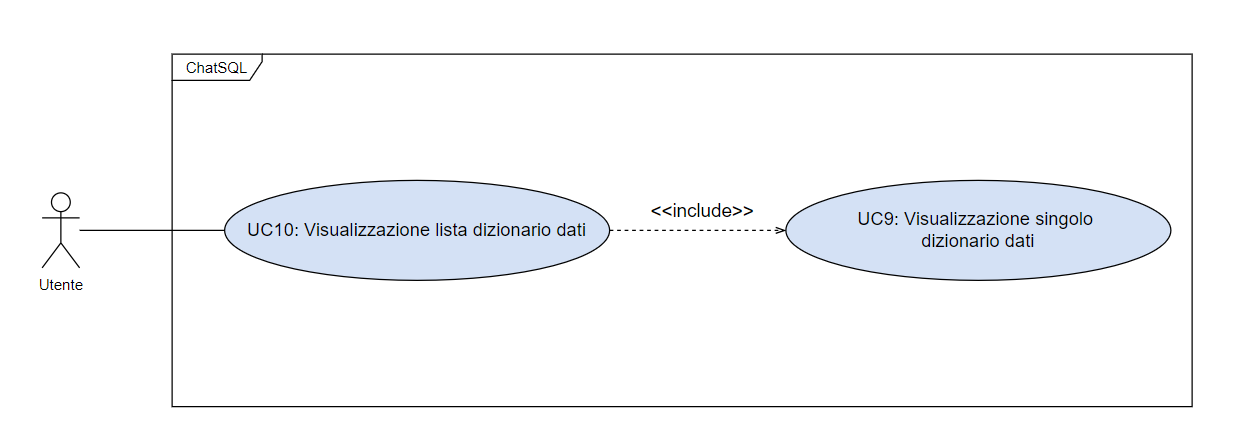
\includegraphics[width=0.90\textwidth]{assets/uc10.png}
  \caption{UC10 - Sottocasi d'uso}
\end{figure}

%%%%%%%%%%%%%%%%%%%%%%%%%%%%%%%%%%%%%%%%%%%%%%%%%%%%%%%%%%%%%%%%%%%%%%%%%%%%%%

\subsubsection{UC10.1 - Visualizzazione nome dizionario dati}\label{UC10point1}
\paragraph*{Descrizione}
L'Utente visualizza il nome di un \glossario{dizionario dati}.

\paragraph*{Attori principali}
Utente

\paragraph*{Precondizioni}
\begin{itemize}
  \item Il sistema è attivo e funzionante;
  \item È stato caricato almeno un \glossario{dizionario dati} nel sistema. 
\end{itemize}

\paragraph*{Postcondizioni}
\begin{itemize}
  \item Viene visualizzato correttamente il nome del \glossario{dizionario dati}.
\end{itemize}

\paragraph*{Trigger}
L'Utente vuole visualizzare il nome di un \glossario{dizionario dati}.

\paragraph*{Scenario principale}
\begin{enumerate}
  \item L'Utente visualizza il nome del \glossario{dizionario dati}.
\end{enumerate}

%%%%%%%%%%%%%%%%%%%%%%%%%%%%%%%%%%%%%%%%%%%%%%%%%%%%%%%%%%%%%%%%%%%%%%%%%%%%%%

\subsubsection{UC10.2 - Visualizzazione estensione dizionario dati}\label{UC10point2}
\paragraph*{Descrizione}
L'Utente visualizza l'estensione di un \glossario{dizionario dati} (es.: .json, .sql).

\paragraph*{Attori principali}
Utente

\paragraph*{Precondizioni}
\begin{itemize}
  \item Il sistema è attivo e funzionante;
  \item È stato caricato almeno un \glossario{dizionario dati} nel sistema. 
\end{itemize}

\paragraph*{Postcondizioni}
\begin{itemize}
  \item Viene visualizzata correttamente l'estensione del \glossario{dizionario dati}.
\end{itemize}

\paragraph*{Trigger}
L'Utente vuole visualizzare l'estensione di un \glossario{dizionario dati}.

\paragraph*{Scenario principale}
\begin{enumerate}
  \item L'Utente visualizza l'estensione del \glossario{dizionario dati}.
\end{enumerate}

%%%%%%%%%%%%%%%%%%%%%%%%%%%%%%%%%%%%%%%%%%%%%%%%%%%%%%%%%%%%%%%%%%%%%%%%%%%%%%

\subsubsection{UC10.3 - Visualizzazione descrizione dizionario dati}\label{UC10point3}
\paragraph*{Descrizione}
L'Utente visualizza la descrizione di un \glossario{dizionario dati}.

\paragraph*{Attori principali}
Utente

\paragraph*{Precondizioni}
\begin{itemize}
  \item Il sistema è attivo e funzionante;
  \item È stato caricato almeno un \glossario{dizionario dati} nel sistema. 
\end{itemize}

\paragraph*{Postcondizioni}
\begin{itemize}
  \item Viene visualizzata correttamente la descrizione del \glossario{dizionario dati}.
\end{itemize}

\paragraph*{Trigger}
L'Utente vuole visualizzare la descrizione di un \glossario{dizionario dati}.

\paragraph*{Scenario principale}
\begin{enumerate}
  \item L'Utente visualizza la descrizione del \glossario{dizionario dati}.
\end{enumerate}

%%%%%%%%%%%%%%%%%%%%%%%%%%%%%%%%%%%%%%%%%%%%%%%%%%%%%%%%%%%%%%%%%%%%%%%%%%%%%%

\subsubsection{UC10.4 - Visualizzazione dimensione dizionario dati}\label{UC10point4}
\paragraph*{Descrizione}
L'Utente visualizza la dimensione di un \glossario{dizionario dati}, che corrisponde al peso del file (es.: 500 KB).

\paragraph*{Attori principali}
Utente

\paragraph*{Precondizioni}
\begin{itemize}
  \item Il sistema è attivo e funzionante;
  \item È stato caricato almeno un \glossario{dizionario dati} nel sistema. 
\end{itemize}

\paragraph*{Postcondizioni}
\begin{itemize}
  \item Viene visualizzata correttamente la dimensione del \glossario{dizionario dati}.
\end{itemize}

\paragraph*{Trigger}
L'Utente vuole visualizzare la dimensione di un \glossario{dizionario dati}.

\paragraph*{Scenario principale}
\begin{enumerate}
  \item L'Utente visualizza la dimensione del \glossario{dizionario dati}.
\end{enumerate}

%%%%%%%%%%%%%%%%%%%%%%%%%%%%%%%%%%%%%%%%%%%%%%%%%%%%%%%%%%%%%%%%%%%%%%%%%%%%%%

\subsubsection{UC10.5 - Visualizzazione data di ultimo aggiornamento dizionario dati}\label{UC10point5}
\paragraph*{Descrizione}
L'Utente visualizza la data di ultimo aggiornamento di un \glossario{dizionario dati}.

\paragraph*{Attori principali}
Utente

\paragraph*{Precondizioni}
\begin{itemize}
  \item Il sistema è attivo e funzionante;
  \item È stato caricato almeno un \glossario{dizionario dati} nel sistema. 
\end{itemize}

\paragraph*{Postcondizioni}
\begin{itemize}
  \item Viene visualizzata correttamente la data di ultimo aggiornamento del \glossario{dizionario dati}.
\end{itemize}

\paragraph*{Trigger}
L'Utente vuole visualizzare la data di ultimo aggiornamento di un \glossario{dizionario dati}.

\paragraph*{Scenario principale}
\begin{enumerate}
  \item L'Utente visualizza la data di ultimo aggiornamento del \glossario{dizionario dati}.
\end{enumerate}